\newpage
\bignumberedpart{Розробка програмного продукту}
\subsection{Синтез алгоритму}

За моделлю Денінга \cite{denning1987intrusion}, компонентами є  % 2 сторінка, овервью

\begin{ESKDexplanation}
\item суб'єкт системи --- абонент, або його телефонний номер;
\item об'єкт системи --- також абонент, друга сторона виклику;
\item записи журналу --- записи, згенеровані внаслідок дій суб'єктів над 
      об'єктами, тобто згенеровані АТС записи CDR;
\item профілі --- структури, згенеровані системою у відповідності до дій 
      суб'єктів над об'єктами, тобто на базі журнальних записів;
\item аномальні записи --- записи CDR, які позначені системою як нехарактерні
      для суб'єкту.
\end{ESKDexplanation}

Виявлення шахрайства в реальному часі базується на гіпотезі, що така поведінка 
включає аномальне використання системи. Тому, шахрайські дії можуть бути 
виявлені як аномальнії у використанні системи. Приклади:
% \cite{denning1987intrusion}.

\begin{itemize}
  \item Клонування телефонів - дані дзвінків перехрещуються у часі, кількість 
        зростає.
  \item Шахрайство при підключенні - до системи підключається новий абонент, 
        шаблон якого ще не побудований (та не зареєстрований в системі). 
        Система дозволяє виявити таких порушників ще до першого зняття коштів з
         рахунку.
  \item Крадіжка телефону - змінюється шаблон поведінки користувача,
  \item Злам АТС - різке збільшення трафіку,
\end{itemize}

Спосіб визначення аномалій за моделлю Деннінга \cite{denning1987intrusion} можна модифікувати так, що змінна 
спостереження - не дискретна величина кількості подій за 
фіксований проміжок часу, а миттєва частота таких подій. Таким 
чином, ми поєднуємо метод числових рядів та статистичного методу
з використанням перших двох моментів розподілу - середнього 
значення та середньоквадратичного відхилення.

Метод \cite{rader2014cdr} полягає в побудові шаблону поведінки користувача на основі декількох тижнів спостереження, і згодом виявлення дзвінків, які виходять за рамки поточного шаблону. Відповідно, робота алгоритму ділиться на 2 етапи: режим навчання і робочий режим.

Враховуючи випадкову природу здійснення телефонного дзвінка по відношенню до оператора, для аналізу поведінки можна виходити з припущення, що кількість дзвінків за певний проміжок часу буде розподілено по розподілу Пуассона.

Також врахуємо, що поведінка користувача залежить від дня тижня. Шаблон поведінки користувача - функція, що показує інтенсивність дзвінків від часу
\begin{equation}\label{eq:pattern_a}P: t \rightarrow \lambda \end{equation}

\begin{ESKDexplanation}
  \item де $\lambda$ - це кількість дзвінків на одиницю часу.
\end{ESKDexplanation}

Тоді запис поведінки користувача можна визначити як вектор довжиною $L = H * 7$, де $H$ - число розбиття доби, а 7 - кількість днів у тижні. У векторі можна зберігати крім значень частоти, також дисперсію з якою було розраховане це значення. Таким чином, кожен елемент шаблону поведінки буде кортежем $(frequency, \sigma)$. Для зменшення випадкової складової, складається декілька записів поведінки по тижнях. Кількість збережених записів $W$ впливає на точність кінцевого шаблону поведінки (\ref{eq:pattern_a})

\begin{equation}\label{eq:pattern_a2}P = (\overline{\lambda_1}, \overline{\lambda_2}, ..., \overline{\lambda_L}) \end{equation}

який можна визначити як усереднений вектор записів поведінки за попередні W тижнів, де середнє значення рахується як експоненціально зважене рухоме середнє з вікном в кількість записів:

\begin{equation}\label{eq:ema}EMA_n = (1-\alpha) \cdot x_n + \alpha \cdot EMA_{n-1} \end{equation}

що можна призвести до не-рекурсивної формули \cite{cargal1988discrete}:

\begin{equation}\label{eq:ema_nonrecursive}EMA = \frac{{x}_{n} + \alpha {x}_{n -1} + {\alpha} ^ {2} {x}_{n -2} +...+ {\alpha} ^ {n -1} {x}_{1}}{1+ \alpha + {\alpha} ^ {2} +...+ {\alpha} ^ {n -1}} \end{equation}

Це дозволяє зменшити запізнювання, надаючи більшого значення останнім значенням.

\begin{equation}\label{eq:ema_lambda}\overline{{\lambda}_{i}} = \frac{{\lambda}_{i w} + \alpha {\lambda}_{i(w -1)} +...+ {\alpha} ^ {n -1} {\lambda}_{i1}}{1+ \alpha + {\alpha} ^ {2} +...+ {\alpha} ^ {w -1}} \end{equation}

У режимі навчання система приймає записи про дзвінки, вимірює частоту дзвінків і фіксує її в записах поведінки. Коли потрібну кількість записів збережено (залежно від обраного критерію, або досягається необхібна дисперсія, або задається необхідна кількість записів), система переводиться в робочий режим для конкретного абонента. Тобто в один момент часу частина абонентів може оброблятися в режимі навчання, а частина - в робочому режимі. Це необхідно, тому що під час роботи системи можуть підключитися нові абоненти.

Підрахунок поточної частоти $\lambda_{r}$ робиться на основі часу ініціації останніх $K$ дзвінків для кожного абонента окремо. Маючи вектор $T_i^{p}, i = \overline{1..K}$ відміток часу ініціації дзвінків (в секундах) розраховуємо передбачувану частоту за певний проміжок часу $T$:

\begin{equation}\label{eq:time_duration} T = \frac{24 \cdot 60 \cdot 60}{H} \end{equation}

Орієнтовна частота за час однієї комірки шаблону:

\begin{equation}\label{eq:one_freq} \lambda_r = T \cdot f \end{equation}
\begin{ESKDexplanation}
  \item де $f$ -- поточна частота за секунду.
\end{ESKDexplanation}

\begin{equation}\label{eq:cur_freq} f = \frac{1}{T_{avg}} \end{equation}
\begin{ESKDexplanation}
  \item де $T_{avg}$ -- середній час між дзвінками
\end{ESKDexplanation}

Для зменшення ефекту запізнювання за зміною частоти, тут також доцільно використовувати експоненційно зважене середнє значення:

\begin{equation}\label{eq:t_avg} T_{avg} = {EMA}_{\alpha}(T_n - T_{n-1}, T_{n-1} - T_{n-2}, ..., T_{2} - T_{1}) \end{equation}

Тоді фактична частота $\lambda_{rt}^p = F(\{T_i^p\})$ (\ref{eq:real_freq}) визначається як:

\begin{equation}\label{eq:cur_freq_final} \lambda_{rt} = \frac{24 \cdot 60 \cdot 60}{H \cdot {EMA}_{\alpha}(T_n - T_{n-1}, T_{n-1} - T_{n-2}, ..., T_{2} - T_{1})} \end{equation}

У робочому режимі система продовжує фіксувати записи поведінки, тобто навчання не зупиняється. У цьому режимі починає працювати алгоритм кластеризації, який класифікує шаблони користувачів на k кластерів. Кількість класів може бути варіювалися для забезпечення точного поділу абонентів за характером використання системи. Для кластеризації можна використовувати алгоритм k-means, що запускається періодично після запису чергового запису поведінки (раз на тиждень), але у зв'язку з його складністю для великої кількості абонентів доцільно використовувати його потокову модифікацію \cite{dasgupta2008clustering}, що дозволить класифікувати шаблони відразу після отримання нових даних.

Крім цього вмикається перевірка кожного дзвінка на відповідність шаблону поведінки. Перевірка на відповідність може здійснюватися як з використанням довірчих інтервалів, так і перевіркою з урахуванням дисперсії. Нехай передбачуваний довірчий інтервал $(f_{min}, f_{max})$ (\ref{eq:denning_confidence}) з необхідною надійністю, що задається оператором, а відхилення поточної частоти (\ref{eq:cur_freq_final}) від передбачуваного значення для інтенсивності розглянутого часового проміжку $\lambda_i$ з шаблону поведінки $P$ (\ref{eq:pattern_freq}):

\begin{equation}\label{eq:div} d = \frac{\lambda_r^i - \lambda_i^p}{f_{max} - f_{min}} \end{equation}
\begin{ESKDexplanation}
  \item де $i$ -- номер комірки шаблону
\end{ESKDexplanation}

Тоді при $-1 \le d \le 1$ значення поточної частоти знаходиться в межах очікуваної.
Для усталеного стану системи, середнє значення відхилень:

\begin{equation}\label{eq:trend} trend_{C} = \sum{\frac{d_i^C}{N^C}} \end{equation}
\begin{ESKDexplanation}
  \item де $i$ -- номер абоненту класу $C$
\end{ESKDexplanation}

буде близький до нуля.

Якщо ж відбуватиметься сезонна зміна або деякий інший фактор, який впливає на характер використання системи класу або декількох класів користувачів, тренд покаже характер цих змін.

Сенсом функції тренду є відсоток відхилення класу абонентів від попереднього характеру використання системи. Тому, для зменшення помилкових спрацьовувань системи виявлення аномального поведінки, необхідно розширити довірчий інтервал на обчислений тренд.

Таким чином, інтервенція може бути виявлена порівнянням поточної частоти з межами довірчого інтервалу (\ref{eq:div}), що дорівнює:

\begin{equation}\label{eq:conf_interval_w_trend} 
  \begin{cases}
    (f_{min}, f_{max} \cdot (1 + |trend|)), & trend > 0;\\
    (f_{min} \cdot (1 - |trend|), f_{max}), & trend < 0.
  \end{cases}
\end{equation} % как считать этот 

Збираючи всі частини разом, отримуємо алгоритм:

\begin{algorithm}[H]
\KwData{Джерело CDR записів}
\KwResult{Сигнали про інтервенції}
% \SetAlgoLined

  \While{є нові записи CDR} {
    \If{шаблон в робочому режимі} {
      \If{CDR не відповідає шаблону} {
        сигнал про інтервенцію\;
       }
    }
   модифікувати шаблон поведінки\;
   перерахувати миттєву інтенсивність\;
   перерахувати тренд\;
   \If{пройшов час $T_{c}$ з останньої кластеризації} {
    ініціювати кластеризацію абонентів\;
   }
  }
\caption{Алгоритм визначення аномальної поведінки}
\label{alg:general_anomaly_detection}
\end{algorithm}

\begin{ESKDexplanation}
  \item де $T_{c}$ - час з останньою кластеризації. Рекомендований час - один тиждень, у ніч з останнього на перший день тижня, коли шаблони поведінки заповнені рівномірно.
\end{ESKDexplanation}

Останній пункт може бути модифікований для потокової кластеризації \cite{dasgupta2008clustering}.


\subsection{Реалізація прототипу системи}
\label{poc-implementing}
Вхідними даними для алгоритму є журнал записів CDR. Такі дані не представлені у відкритому доступі, тому що вони є конфіденційні.

Для перевірки роботи системи був написаний імітатор записів CDR. Можливості програми дозволяють імітувати активність скінченої кількості користувачів, що роблять дзвінки за шаблонами поведінки із додаванням випадкового шуму.

Прототип складається із двох частин:
\begin{enumerate}
\item Імітатор - складова, що емулює реальну АТС;
\item Аналізатор - реалізація алгоритму \ref{alg:general_anomaly_detection} визначення аномальної поведінки.
\end{enumerate}

Шаблон поведінки - вектор $P = (\overline{\lambda_1}, \overline{\lambda_2}, \dots, \overline{\lambda_L})$ (\ref{eq:pattern_a2}), де в даній конкретній реалізації:

\begin{equation}\label{eq:l_count}L = 7 \cdot 24 = 168 \end{equation}

Кожна комірка є інтенсивністю дзвінків на секунду (\ref{eq:ema_lambda}).

Імітатор генерує записи для $N$ абонентів для кожного з $k$ класів, що задаються перед запуском. Кожному абоненту співставляється шаблон його поведінки. Дзвінки від кожного абоненту є неоднорідним пуасонівським потіком, інтенсивність якого залежить від часу та береться із шаблону поведінки $P$:

\begin{equation}\label{eq:puasson}\lambda_p(t) = P^p_{hourOfWeek(t)} \end{equation}

\begin{ESKDexplanation}
  \item де $p$ - це ідентифікатор абоненту,
  \item $hourOfWeek(t)$ - функція, що повертає номер години з початку тижня. $1 \le hourOfWeek(t) \le L$.
\end{ESKDexplanation}

Аналізатор приймає кожний запис CDR і послідовно перевіряє його на аномальність, враховує новий запис для поточної інтенсивності, змінює шаблон поведінки і при необхідності запускає кластеризацію. Загальна функціональна схема розробленого прототипу на \autoref{fig:poc-scheme}.

Аналізатор, як і імітатор, написані мовою Python 3, використовують бібліотеки sklearn для кластеризації абонентів та matplotlib для візуалізації графіків. Для кластеризації використовується алгоритм k-means.

\begin{figure}[h]
        \begin{center}
            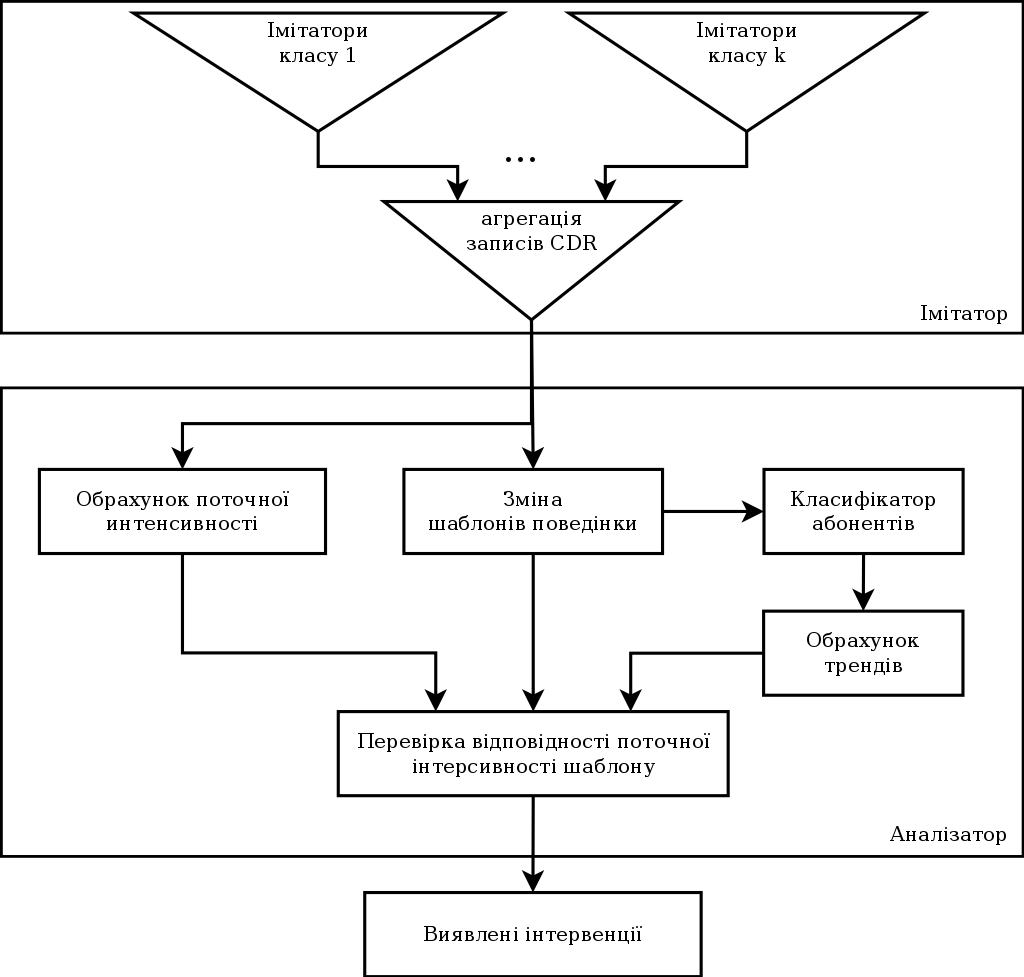
\includegraphics[scale=0.4]{resources/System-mini.png}
        \end{center}
        \caption{Функціональна схема прототипу системи}
        \label{fig:poc-scheme}
\end{figure}

Вихідний код прототипу у додатку \TBD.

\subsection{Модифікація алгоритму для роботи в паралельній комп'ютерній системі}

\label{parallel}
Після написання прототипу за алгоритмом \ref{alg:general_anomaly_detection}, були виявлені недоліки прямої реалізації алгоритму (результати моделювання у розділі \ref{poc}):
\begin{itemize}
\item Розрахунок шаблонів ведеться в одному потоці із перевіркою запису CDR, що збільшує кількість обчислень для обробки одного запису CDR та збільшує потреби до оперативної пам'яті; через деякий час робочий шаблон має бути замінений на розрахований;
\item Кластеризація абонентів ведеться в одному потоці із перевіркою запису CDR, що дає суттєву затримку раз на тиждень;
\item Розрахунок тренду не враховує маштабування системи, вимагає копіювання шаблонів на кожну машину, на якій розраховується тренд (тобто на всіх машинах, що обробняють CDR) або потребує системи із загальною пам'яттю;
\item Враховуючи вищезгадане, алгоритм не забеспечує константного часу обробки.
\end{itemize}
% список недоліків: типу, довго працює, тому що в тому ж потоці рахує шаблони та кластеризує

Крім цього, в прототипі імітатор суміщений із системою виявлення аномалій, що не дає змогу використовувати продукт у реальній виробничій системі. Для вирішення цього питання між АТС та системою виявлення аномалій має бути встановлене проміжне програмне забеспечення для доставки повідомлень, яке буде буфером.

Враховуючи запит на найшвидше реагування в реальному часі, алгоритм має бути декомпозований на частини та система має бути спроектована із врахуванням маштабування.

Алгоритм складається із таких умовно незалежних частин: \label{parts_of_algorithm}

\begin{itemize}
\item Кластеризація абонентів,
\item Розрахунок шаблонів поведінки,
\item Перевірка записів CDR на аномальність.
\end{itemize}

Кластерізація та розрахунок шаблонів поведінки це важкі обчислення, які не потребують обробки в реальному часі але потребують обробки великого обсягу журналу, тому їх можна винести у окрему періодичну задачу. Такі задачі добре розв'язуються за допомогою парадігми Map-Reduce.

Перевірка записів CDR на аномальність є єдиною частиною, до якої висуваються вимоги реального часу.

Необхідно також забеспечити розрахунок трендів в рамках задачі перевірки на аномальність. Враховуючи необхідність доступу до всіх миттєвиї частот в межах класу користувачів на даний момент при розрахуванні тренду, що означає необхідність забеспечення загальної пам'яті, необхідно забеспечити швидке сховище для таких даних. Ця задача потребує особливих оптимізацій щоб не бути вузьким місцем у паралельному алгоритмі.

\subsection{Архітектура системи}

\subsubsection{Проектування системи}

Система має дві логічні частини, зображені у правій частині \autoref{fig:struct-scheme-overview}:
\begin{itemize}
\item Частина реального часу для швидкої перевірки вхідних записів CDR,
\item Періодична частина, що обробляє всю історію журналу CDR за останні чотири тижні. % надо посчитать!!!!!!! сколько там данных реально
\end{itemize}

На \autoref{fig:struct-scheme-overview} зображені усі компоненти, що мають бути присутніми у системі для забеспечення всіх вимог.

\begin{figure}[h]
        \begin{center}
            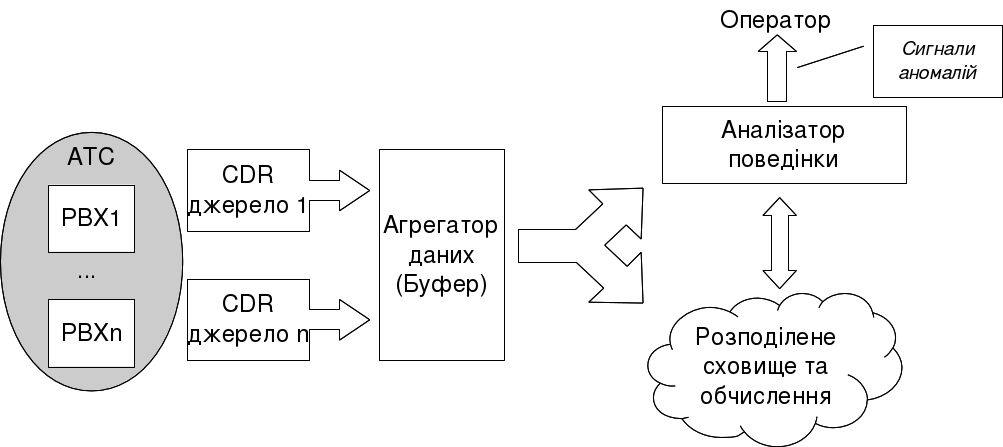
\includegraphics[scale=0.65]{resources/struct-1.png}
        \end{center}
        \caption{Структура системи}
        \label{fig:struct-scheme-overview}
\end{figure}

Періодична частина включає в собі дві задачі, кластеризацію та розрахунок шаблонів поведінки. Для розрахунку шаблонів поведінки потрібно опрацювати історію за останні 4 тижні. Цей об'єм даних потрібно також зберігати. Для цього необхідно забеспечити в системі маштабований компонент для зберігання та обрахунку великих об'ємів даних.

Для перевірки вхідних записів CDR має бути забеспечена велика пропускна здатність. Це має бути окремий компонент системи, що не залежить від сховища даних щоб затримка від потрапляння запису у систему до обробки його була мінімальною. Тобто система доставки повідомлень має одночасно доставляти повідомлення двом приймачам:

\begin{itemize}
\item аналізатору поведінки для перевірки запису CDR на аномальність;
\item приймачу в розподілене сховище даних для подальшого обрахунку шаблонів поведінки.
\end{itemize}

На \autoref{fig:struct-scheme-tasks} зображені компоненти системи, а також задачі що вони мають виконувати.

\begin{figure}[h]
        \begin{center}
            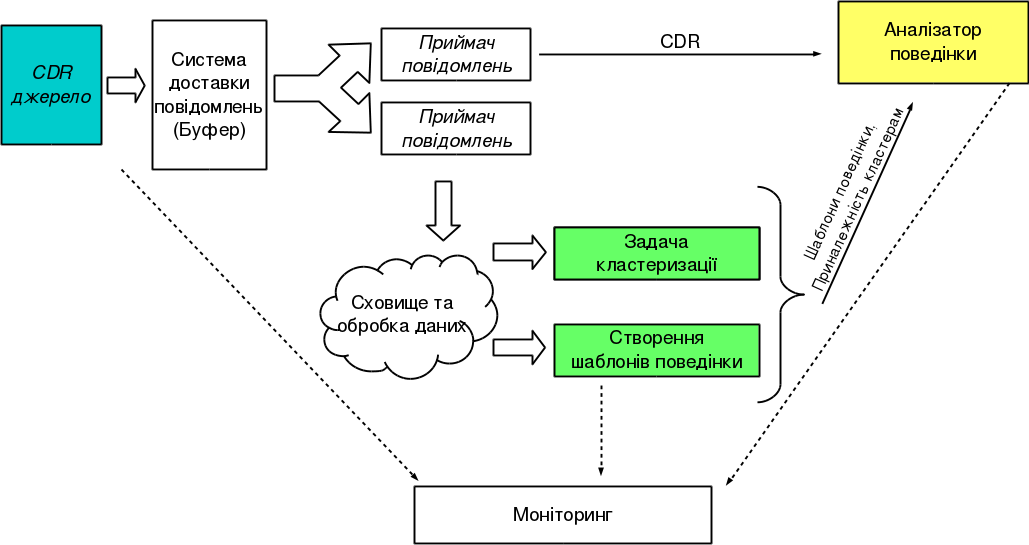
\includegraphics[scale=0.6]{resources/struct-2.png}
        \end{center}
        \caption{Задачі, що виконують компоненти системи}
        \label{fig:struct-scheme-tasks}
\end{figure}

\subsubsection{Журнал дзвінків}
  Вхідний потік подій ${T_i^p}$ складається із записів даних виклику, модель 
  даних записів - CDR - Call Detail Record. В кожен запис входять такі поля (в 
  дужках позначені назви комірок у системі АТС Asterisk):

   \begin{itemize}
    \item номер абонента, що ініціював дзвінок (src);
    \item номер абонента, кому був адресований дзвінок (dst);
    \item час ініціювання дзвінка (start);
    \item час відповіді на дзвінок (answer);
    \item час завершення дзвінку (end);
    \item довжина дзвінку -- різниця між полями end та start (duration);
    \item довжина розмови -- різниця між полями end та answer (billsec);
    \item статус дзвінка -- прийнятий, відхилений, зкинутий, інше (disposition).
  \end{itemize}

  Статус дзвінка може приймати значення

  \begin{itemize}
    \item NO ANSWER --- адресат не прийняв дзвінок;
    \item FAILED --- невідомий адресат або інша помилка системи/ліній зв'язку;
    \item BUSY --- лінія адресата зайнята / адресат скинув дзвінок;
    \item ANSWERED --- успішний дзвінок;
    \item UNKNOWN --- статус невідомий.
  \end{itemize}

  може бути розширений в залежності від використовуваних інструментів та аппаратного/програмного забеспечення АТС.

  \begin{table}[h]
  \footnotesize
  \caption{Приклад журналу CDR}
        \begin{tabularx}{\textwidth}{| X | X | X | X | X | X | X | X |}
          \hline
          Абонент що дзвонить & Абонент що викликається & Ініц. дзвінка (с) & Від-повідь (с) & Кінець (с) & Три-валість (с) & Три-валість розмови (с) & Статус \\ \hline
          \scriptsize{0000000244} & \scriptsize{0007679961} & 365996 & 366049 & 366095 & 99 & 46 & \scriptsize{ANSWERED} \\ \hline
          \scriptsize{0000000238} & \scriptsize{0000434356} & 376215 & 376230 & 376354 & 139 & 124 & \scriptsize{ANSWERED}  \\ \hline
      \end{tabularx}
      \label{tab:cdr-log-example}
  \end{table}


\subsection{Вибір інструментів для реалізації системи}

Для розробки системи, схема якої зображена на \autoref{fig:struct-scheme-tasks} потрібно вибрати інструменти для наступних задач:

  \begin{itemize}
    \item Обробка та зберігання журналів CDR;
    \item Швидкий аналіз записів CDR;
    \item Система доставки повідомлень.
  \end{itemize}

Для обробки та зберігання таких об'ємів інформації як журнали CDR % яких??
обране програмне забеспечення Apache Hadoop.

Програмна бібліотека Apache Hadoop є основою, яка дозволяє розподілено обробляти великі масиви даних на кластері комп'ютерів за допомогою простих моделей програмування. Він призначений для маштабування від одиночних серверів до тисячей машин, кожна з яких дозволяє локальні обчислення та зберігання даних. Замість того, щоб покладатися на обладнання, що дозволяє високу доступність, сама бібліотека призначена для виявлення і обробки збоїв на рівні додатків, тому бібліотека постачає ПЗ на базі Hadoop послуги високої доступності на кластері комп'ютерів, кожен з яких може бути схильний до невдач.

ПЗ Apache Hadoop дозволяє розв'язати задачі зберігання великих об'ємів даних на розподіленій файловій системі HDFS, а також надає можливість написання додатків для обробки цих даних за допомогою парадигми MapReduce, що дозволяє ефективно паралелити обчислення на рівні бібліотеки.

Для швидкого аналізу даних обрана система розподіленого обчислення в реальному часі Apache Storm.

Apache Storm є вільним ПЗ з відкритим вихідним кодом, це розподілена система обчислення в реальному часі. Storm дозволяє легко та надійно обробляти необмежені потоки даних, роблячи для обробки в реальному часі те саме, що Hadoop зробив для пакетної обробки.

Шторм має багато варіантів використання: аналітика в реальному часі, машинне навчання, безперервне обчислення, розподілених RPC, ETL, і багато іншого. Storm швидкий: є заміри, щоо показують результат в понад мільйон оброблюваних кортежів за секунду на вузол. Рішення є масштабованим, відмовостійким, гарантує що дані будуть оброблені.

Для доставки повідомлень необхідне ПЗ що забеспечує персистентну розподілену чергу, що може розповсюджувати повідомлення кільком приймачам. Для цього обране ПЗ Apache Kafka, що використовує в своїй основі Apache Zookeeper як розподілене сховище типу ключ-значення. Це сховище вже використовуєтсья в стеку ПЗ Apache Hadoop, тому є сенс використати саме Kafka.

Apache Kafka - система публікації-підписки повідомлень, як розподілена система зберігання данних журналів. Один брокер Kafka може обробляти сотні мегабайт в секунду від тисяч клієнтів.

Kafka розроблена, щоб використовувати один кластер як центральну магістраль даних для великої організації. Він може бути легко і прозоро маштабований без простоїв. Потоки даних розділені і розподілені по кластерам машин, щоб дозволити збільшити пропускну здатність, ніж можливості будь-якої окремої машини і дозволити кластерам координувати споживачів.

Повідомлення зберігаються на диску і відтворюються в рамках кластера, щоб запобігти втраті даних. Kafka має сучасну архітектуру кластера, що гарантує відмовостійкість.

Додатково має бути розроблена система моніторингу. Для зберігання даних необхідне швидке сховище, до якого не виносяться вимоги по персистентності даних. Таким сховищем може бути Redis.  Redis є ПЗ з відкритим вихідним кодом, BSD ліцензією, що є сховищем типу ключ-значення. Redis часто згадується як сервер структури даних так як ключі можуть містити рядки, хеши, списки, набори і сортовані набори.
\begin{figure}[h]
        \begin{center}
            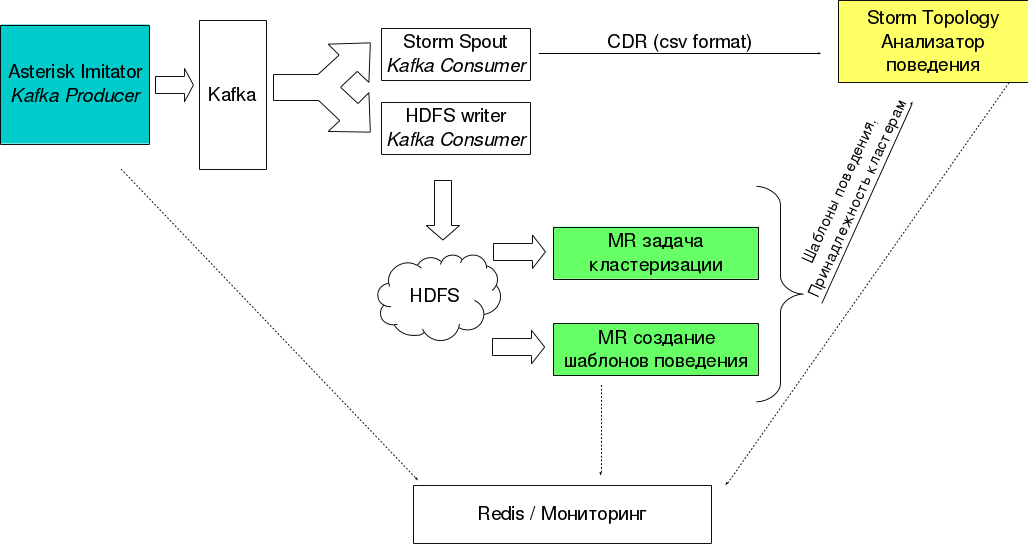
\includegraphics[scale=0.6]{resources/struct-3.png}
        \end{center}
        \caption{Компоненти системи з обраними інструментами}
        \label{fig:struct-scheme-components}
\end{figure}

Всі використані інструменти з відкритим вихідним кодом та розповсюджуються за ліцензією Apache License 2.0 та BSD, що дозволяє використовувати їх в даній дипломній роботі. Всі обрані компоненти позначені на \autoref{fig:struct-scheme-components}.

\subsection{Розробка програмного продукту}

\subsubsection{Імітатор АТС}

Імітатор написаний мовою Java, основні можливості збігаються із можливостямі імітатора прототипу в розділі \ref{poc-implementing}.

Можливості імітатора:
\begin{itemize}
  \item Імітація одного телефонного абоненту (\autoref{fig:imit-1});
  \item Імітація багатьох абонентів одного класу (із схожим шаблоном використання мережі) (\autoref{fig:imit-2});
  \item Імітація багатьох абонентів багатьох класів (\autoref{fig:imit-3});
  \item Можливість внести інтервенцію в роботу будь-якої кількості абонентів.
\end{itemize}

\begin{figure}[h]
        \begin{center}
            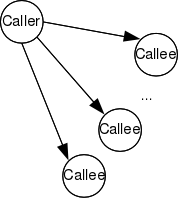
\includegraphics[scale=0.8]{resources/imit-1.png}
        \end{center}
        \caption{Один абонент, один шаблон}
        \label{fig:imit-1}
\end{figure}

\begin{figure}[h]
        \begin{center}
            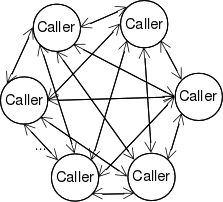
\includegraphics[scale=0.8]{resources/imit-2.png}
        \end{center}
        \caption{Багато абонентів, один шаблон}
        \label{fig:imit-2}
\end{figure}

\begin{figure}[h]
        \begin{center}
            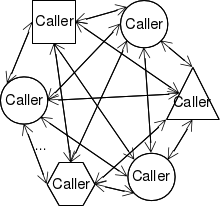
\includegraphics[scale=0.8]{resources/imit-3.png}
        \end{center}
        \caption{Багато абонентів, різні шаблони}
        \label{fig:imit-3}
\end{figure}

Імітатор генерує записи для $N$ абонентів для кожного з $k$ класів, що задаються перед запуском. Кожному абоненту співставляється шаблон його поведінки. Дзвінки від кожного абоненту є неоднорідним пуасонівським потіком, інтенсивність якого залежить від часу та береться із шаблону поведінки $P$:

\begin{equation}\label{eq:puasson}\lambda_p(t) = P^p_{\lambda, hourOfWeek(t)} \end{equation}

\begin{algorithm}[h]
\KwData{N -- кількість записів для генерації; n -- кількість імітованих абонентів; k -- кількість класів; $\{P_i\}, i \in \overline{1..k}$ -- шаблони поведінки всіх абонентів; $T_{start}$ -- час першого запису}
\KwResult{Записи CDR журналу}
% \SetAlgoLined
  Створити коллекцію шаблонів($\{P_i\}$, n, k)\;
  \For{i=1 \KwTo $N$}{
    \ForEach{$p$ в колекції шаблонів}{
      \If{група подій у $p$ - найближча до поточного часу}{
        $P = p$\;
      }
    }
    
    \ForEach{$c$ в колекції абонентів $P$}{
      \If{подія у $c$ - найближча до поточного часу}{
        $C = c$\;
      }
    }
    $CDR$ = Створити запис CDR для абоненту ($C$, $T_{start}$)\;
    $next$ = Розрахувати наступну подію абоненту $C$\;
    Запам'ятати $next$ як час найближчої події для $P$\;

    Вивід($CDR$)\;
  }
\caption{Алгоритм роботи імітатора АТС}
\label{alg:imitator}
\end{algorithm}

Скорочена діаграма класів, що реалізують бізнес-логіку розробленого імітатора на \autoref{fig:imit-uml-classes}.

\begin{figure}[h]
        \begin{center}
            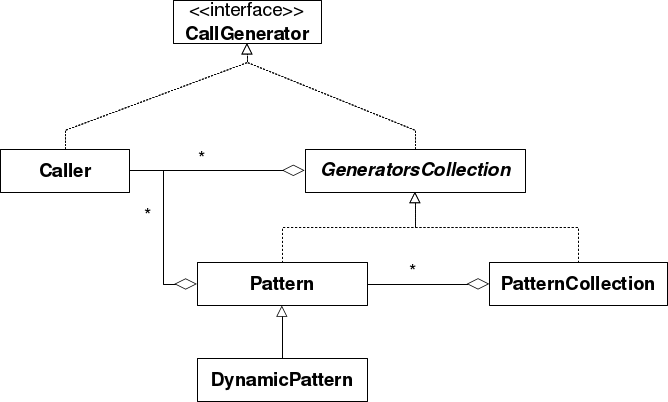
\includegraphics[scale=0.8]{resources/imit-uml-classes.png}
        \end{center}
        \caption{Скорочена діаграма основних класів, що реалізують бізнес-логіку}
        \label{fig:imit-uml-classes}
\end{figure}

Алгоритм роботи імітатора приведений в алгоритмі \ref{alg:imitator}. Приклад однієї ітерації роботи імітатора зображено на діаграмі послідовності \autoref{fig:imit-uml-1}.

\begin{figure}[h]
        \begin{center}
            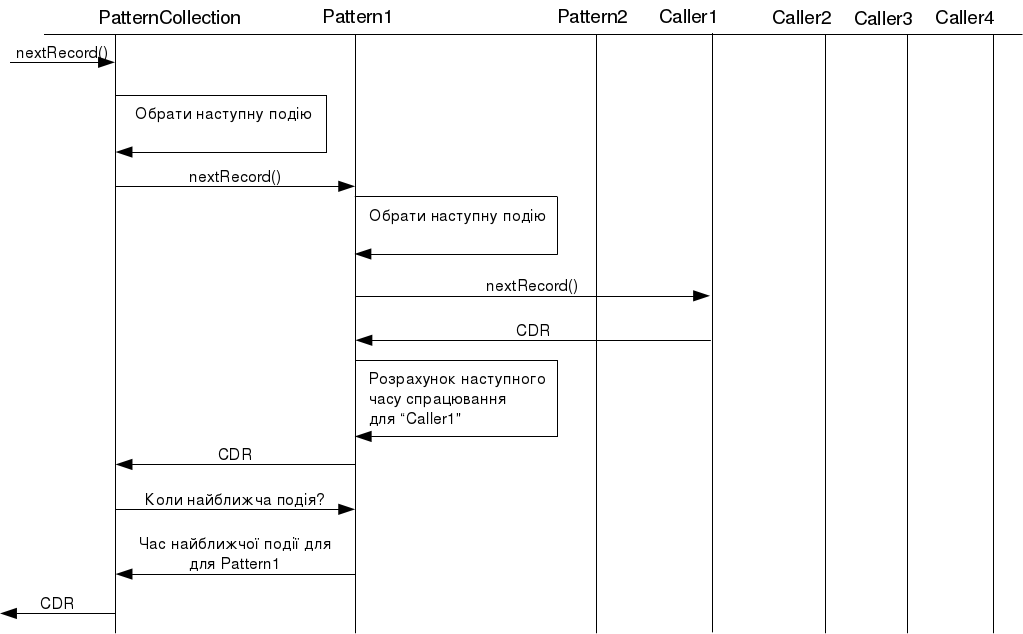
\includegraphics[scale=0.6]{resources/imit-uml.png}
        \end{center}
        \caption{Приклад однієї ітерації роботи імітатора}
        \label{fig:imit-uml-1}
\end{figure}


Також головною відмінністю від прототипу є те, що імітатор є незалежним компонентом, що має свою точку входу. Імітатор може використовувати декілька інтерфейсів для видачі результатів генерації:

\begin{itemize}
  \item Інтерфейс Kafka Producer, тобто завантажуючи згенеровані записи прямо в розподілену систему доставки повідомлень, він використовується у робочому режимі системи;
  \item Видача результатів у стандартний вивід: до файлу або у інтерпретатор командного рядку, такий інтерфейс використовується при тестуванні для генерації тестового набору даних;
  \item Інтерфейс Storm Spout, тобто завантажуючи згенеровані записи у топологію Storm - такий інтерфейс використовується при тестуванні для генерації перевірочного набору даних.
\end{itemize}

\subsubsection{Аналізатор поведінки}

Аналізатор поведінки є програмою, написаню мовою Java із використанням фреймвору Apache Storm і призначеною для для запуску на кластері Storm.

Основним елементом, що оброблює записи CDR є ProcessBolt (\autoref{fig:topology-test} та \autoref{fig:topology-prod} - Аналізатор). Для перевірки запису на аномальність необхідно мати шаблони поведінки всіх користувачів та результати кластеризації. Ця інформація знаходиться на HDFS в робочому режимі та на файловій системі локального комп'ютера в тестовому режимі.

Тут джерелом CDR записів виступає Storm Spout, що у тестовому режимі є імітатором АТС, а у робочому режимі є Kafka Consumer, що читає дані із черги Kafka.

\begin{algorithm}[h]
\KwData{Джерело CDR записів}
\KwResult{Сигнали про інтервенцію}
% \SetAlgoLined
  Завантажити шаблони користувачів та класи\;
  
  \While{є нові записи CDR} {
    $CDR = $ прочитати новий запис\;
    $P$ = шаблон поведінки для $CDR.src$\;
    \If{шаблон $P$ в робочому режимі} {
      \If{$CDR$ не відповідає шаблону} {
        сигнал про інтервенцію\;
       }
    }
   перерахувати миттєву інтенсивність\;
   перерахувати тренд\;
  }
\caption{Алгоритм роботи аналізатора}
\label{alg:analysis}
\end{algorithm}

В алгоритмі роботи аналізатора (алгоритм \ref{alg:analysis}) перевірка чи є шаблон в робочому режимі є обмеженням середнього середньоквадратичного відхилення зверху константним значенням $\sigma_{max}$, що задається оператором. В моделюванні це значення дорівнює $\sigma_{max} = 5$.

\begin{equation}\label{eq:isConverged} \overline{\sigma^P} = \frac{1}{168} \cdot \sum_{i=1}^{168}{\sigma^P_i} < \sigma_{max} \end{equation}

Розрахунок відхилення від шалону виконується за модифікованою формулою (\ref{eq:div}):

\begin{equation}\label{eq:deviation_real} d = \frac{f_{current} - f_{pattern}}{2 \cdot 1.96 \cdot \sigma_{pattern}} \end{equation}

Виходячи із припущення, що значення частоти по тижнях розподілені за нормальним розподілом, приймаючи довірчий інтервал у $95\%$, різниця між верхньою і нижньою границею довірчого інтервалу буде $2 \cdot 1.96 \cdot \sigma_{pattern}$. Тоді:

\begin{equation}\label{eq:deviation_real} d = \frac{f_{current} - f_{pattern}}{2 \cdot 1.96 \cdot \sigma_{pattern}} \end{equation}

Після кожних k прийнятих записів CDR поточне значення $d$ записується у сховище Redis для кожного абоненту з ключами <<currentFrequency: <cluster>: <src> >> окремо та розраховуються значення тренду виходячи із записів Redis за формулою (\ref{eq:trend}), а власне перевірка відбувається на входження значення $\lambda_{cur}$ у інтервал, розрахований за (\ref{eq:conf_interval_w_trend}), або якщо використовувати як базу значення $d$, метод підрахунку границь, що базується на використання середньоквадратичного відхилення і $95\%$ довірчого інтервалу, буде:

\begin{equation}\label{eq:conf_interval_w_trend_real} 
  d \in \begin{cases}
    (-1; 1 + trend_{C}), & trend_{C} > 0;\\
    (-1 - trend_{C}; 1), & trend_{C} < 0;
  \end{cases}
  .
\end{equation} % как считать этот 

де $\lambda_{cur}$ розраховується як експоненційно зважене середнє (\ref{eq:cur_freq_final}) ($\alpha = 0.8$) для зглажування піків та зменшення запізнювання за реальним значенням.

\begin{figure}[h]
        \begin{center}
            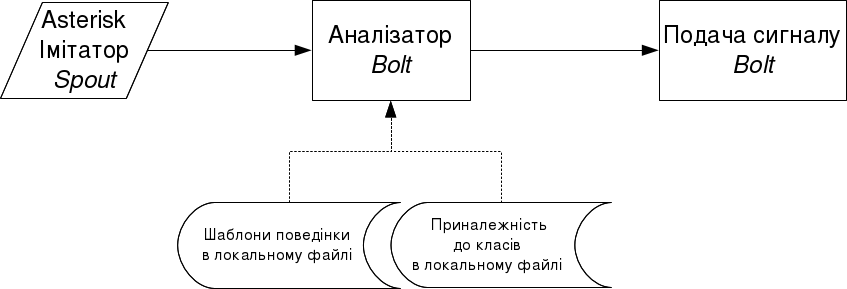
\includegraphics[scale=0.6]{resources/analys-1.png}
        \end{center}
        \caption{Топология Storm детектора аномальної поведінки в режимі тестування}
        \label{fig:topology-test}
\end{figure}

\begin{figure}[h]
        \begin{center}
            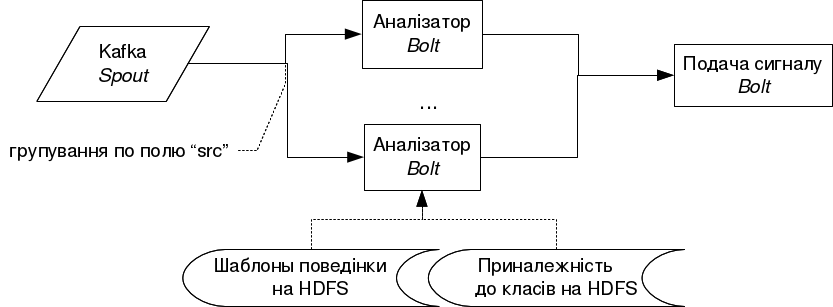
\includegraphics[scale=0.7]{resources/analys-2.png}
        \end{center}
        \caption{Топология Storm детектора аномальної поведінки в робочому режимі}
        \label{fig:topology-prod}
\end{figure}

\subsubsection{Програма кластеризації абонентів}

Для кластеризації абонентів використаний алгоритм k-means++, що дозволяє розділити абонентів на k необхідних груп. Програма написана мовою Python, може працювати в кластері Hadoop з використанням утиліти Hadoop Streaming, що дозволяє запускати MapReduce задачі задаючи Mapper та Reducer із зовні.

Також є можливість запуску програми у локальному режимі, без використання Hadoop.

Розрахунок початкових кластерів приведений на алгоритмі \ref{alg:clustering_init}. Після розрахунку початкових кластерів використовується звичайний агоритм k-means, кількість ітерацій задається перед запуском. Використання покращеної ініціалізації (замість задання випадкових початкових точок) дає можливість суттєво зменшити кількість ітерацій, що важливо при роботі із кластером Hadoop, де кожна ітерація є окремою задачею та має великі накладні витрати на запуск.

\begin{algorithm}[h]
\KwData{$N_{centers}$ -- кількість центрів; ${P_i}$ -- множина шаблонів}
\KwResult{$N_{centers}$ початкових центрів кластерів}
% \SetAlgoLined
  \For{i=1 \KwTo $N_{centers}$} {
    \eIf{жодного центру ще не знайдено} {
      $C_{0} = P_{0}$\;
    }{
      maxDist = 0\;
      \ForEach{$p$ із ${P}$} {
        \ForEach{$c$ із $C$} {
          dists[i] = Евклидова відстань($p$, $c$)\;
        }
        dist = min(dists)\;
        \If{dist > maxDist} {
          fCenter = запам'ятати новий претендент на центр\;
          maxDist = dist\;
        }
      }
      додати до $C$ новий центр fCenter\;
    }
  }
\caption{Алгоритм розрахунку початкових кластерів}
\label{alg:clustering_init}
\end{algorithm}

Програма має запускатися періодично, раз на тиждень, одразу після завершення обчислення шаблонів поведінки (розділ \ref{patterns_section}).

\subsubsection{Програма створення шаблонів поведінки користувачів}
\label{patterns_section}

Для побудови шаблонів поведінки необхідно опрацювати журнал CDR за останніх кількі місяців, або більше за необхідністю. Програма написана мовою Apache Pig, що дозволяє писати програми в парадигмі MapReduce використовуючи такі високорівневі засоби як групування.

\begin{algorithm}[h!]
\KwData{${CDR}$ -- дані журналу CDR}
\KwResult{${P}$ -- шаблони поведінки абонентів}
data = завантажити модель даних та задати формат\;
last = час останнього запису в data\;
dataOperational = фільтрувати data за останній місяць: $(start > last - 4*7*24*60*60)$\;
D = \ForEach{d в dataOperational} {
  $hourOfDay = hourOfDay(d.start)$, $weekDay = weekDay(d.start)$, $weekNumber = weekNumber(last - d.start)$\;
}
times = \ForEach{з групи D за полями $src, hourOfDay, weekDay$} {
  $id = group.weekDay*24+group.hourOfDay$\;
  $freq = EMA(count(D.weekNumber)), \alpha = 0.8$\;
}
data1week = фільтрувати записи D, де weekNumber = 1\;
times1week = \ForEach{з групи data1week за полями $src, hourOfDay, weekDay$} {
  $id = group.weekDay*24+group.hourOfDay$\;
  $count = count(data1week)$\;
}
sigma = \ForEach{з групи times та times1week за полями $src, id$} {
  $\sigma^{id} = \sqrt{\frac{1}{n} \sum{({times}^{id}_i - {times1week}^{id}_i)^2}}$\;
}
patterns = згрупувати sigma та times за полями $src, id$\;
Записати шаблони поведінки patterns у сховище даних\;
\caption{Алгоритм розрахунку шаблонів поведінки}
\label{alg:patterns}
\end{algorithm}

Були написані UDF (User Defined Functions) мовою Python для розрахунку експоненційно зваженого середнього та кілька допоміжних функцій, що використовуються в програмі Pig для розширення функціональності.

Згідно із алгоритмом \ref{alg:patterns}, шаблон поведінки у результаті обробки являє собою два вектори довжиною в 168 елементів, перший з яких є усереднений за формулою (\ref{eq:ema_lambda}) вектор з кількістю дзвінків за кожну годину тижня, а другий вектор - середньоквадратичне відхилення відповідного розрахованого значення з першого вектору.

Проміжні результати обчислень зберігаються на HDFS, а не в оперативній пам'яті, що дозволяє широко маштабувати обчислення та обчислювати об'єми більші, ніж це було б можливо із використанням однієї машини.

Програма має запускатися періодично, раз на тиждень.

\subsubsection{Моніторинг системи}

Окремо розроблений додаток для моніторингу всієї системи. Програма є веб-додатком, написана мовою Python з використанням фреймворку Django. Дозволяє відображати шаблони поведінки абонентів у вигляді теплової карти (\autoref{fig:monitor-1}) та графіки аналізу їх поведінки (\autoref{fig:monitor-2}). Абоненті, що були кластеризовані різними у різні групи відображаються різними кольорами.

Дані що відображаються знаходяться у базі даних Redis, що є in-memory сховищем типу ключ-значення та потраплають туди завдяки засобам моніторингу, вбудованих в інші компоненти системи, такі як аналізатор поведінки та програму створення шаблонів поведінки.

\begin{figure}[h]
        \begin{center}
            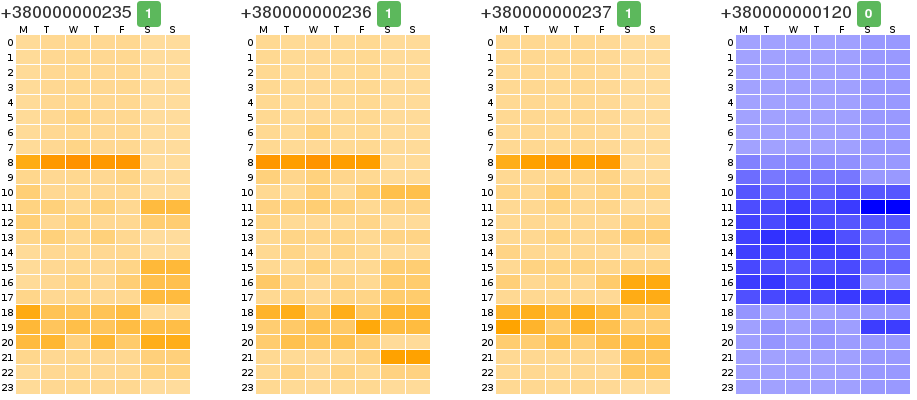
\includegraphics[scale=0.4]{resources/monitor-1.png}
        \end{center}
        \caption{Приклад відображення шаблонів поведінки у вигляді теплової карти}
        \label{fig:monitor-1}
\end{figure}

\begin{figure}[h]
        \begin{center}
            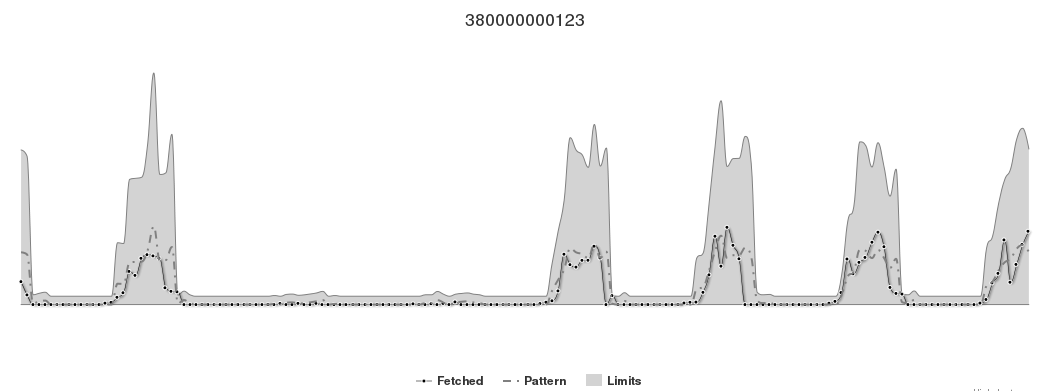
\includegraphics[scale=0.4]{resources/monitor-2.png}
        \end{center}
        \caption{Приклад відображення аналізу поведінки користувача}
        \label{fig:monitor-2}
\end{figure}


\newpage
\subsection*{Висновки до розділу 2}
\addcontentsline{toc}{subsection}{Висновки до розділу 2}

Розроблена система враховує недоліки, які були виявлені у прототипі, дозволяє зберігати та опрацьовувати необмежені об'єми журналів та досягти константного часу опрацювання записів CDR. Забеспечує реплікацію зберігання даних та обробку записів що поступають у реальному часі.

Вимоги реального часу застосовуються для компоненту, що опрацьовує записи CDR що надходять. Основна вимога для роботи в реальному часі, що була не виконана у прототипі це неконстантність часу обробки. В одному потоці із перевіркою на аномальність система рахувала шаблони поведінки та робила кластеризацію абонентів. В розробленій системі час опрацювання одного запису CDR є константним.

До запису в HDFS та періодичним задачам опрацювання журналу CDR вимоги реального часу не висуваються, але швидкість опрацювання всього масиву даних також важливий для найшвидшого введення нових шаблонів в дію після завершення операційного тижня.

Місцем, що лімітує паралелизм є Redis, що дозволяє розподіляти між обчислювальними вузлами поточну частоту для кожного номера абоненту. Але при досягненні максимальної пропускної здатності в цьому місці обмеження можно обійти додавши очікування між оновленням даних в БД кожну кратну кількість отриманих записів. Така затримка в оновленні тренду абсолютно не є критичною, тому що зміна поведінки великим колом користувачів не є моментальна операція, а може відбуватися протягом годин.
